\documentclass{standalone} 
\usepackage{tikz}
\usetikzlibrary{positioning, shapes, automata, arrows}
\usetikzlibrary{shapes.geometric}
\usepackage{pgfplots}
\usepackage{latexsym}
\usepackage{algorithm}
\usepackage{algorithmic}
% \pgfplotsset{compat=latest}
\usepackage{amsmath}
\usepackage[varg]{txfonts}
\usepackage{pgfplotstable}
\usetikzlibrary{patterns}
\def\minYear{1987}
\def\maxYear{2014}
\def\xmin{\minYear-1900-0.5}
\def\xmax{\maxYear-1900+0.5}
\pgfplotsset{compat=1.13}  % PGFPlots 1.13の機能セットを使用することを宣言
% used PGFPlots v1.14
% \documentclass[border=5pt]{standalone}
% \usepackage{pgfplots}
\usetikzlibrary{
       patterns,
}
       \pgfplotsset{
           compat=1.7,
           % define your own legend style here
           my ybar legend/.style={ 
             legend image code/.code={
               \draw [##1] (0cm,-0.6ex) rectangle +(2em,1.5ex);
               },
           },
       }
\begin{document}
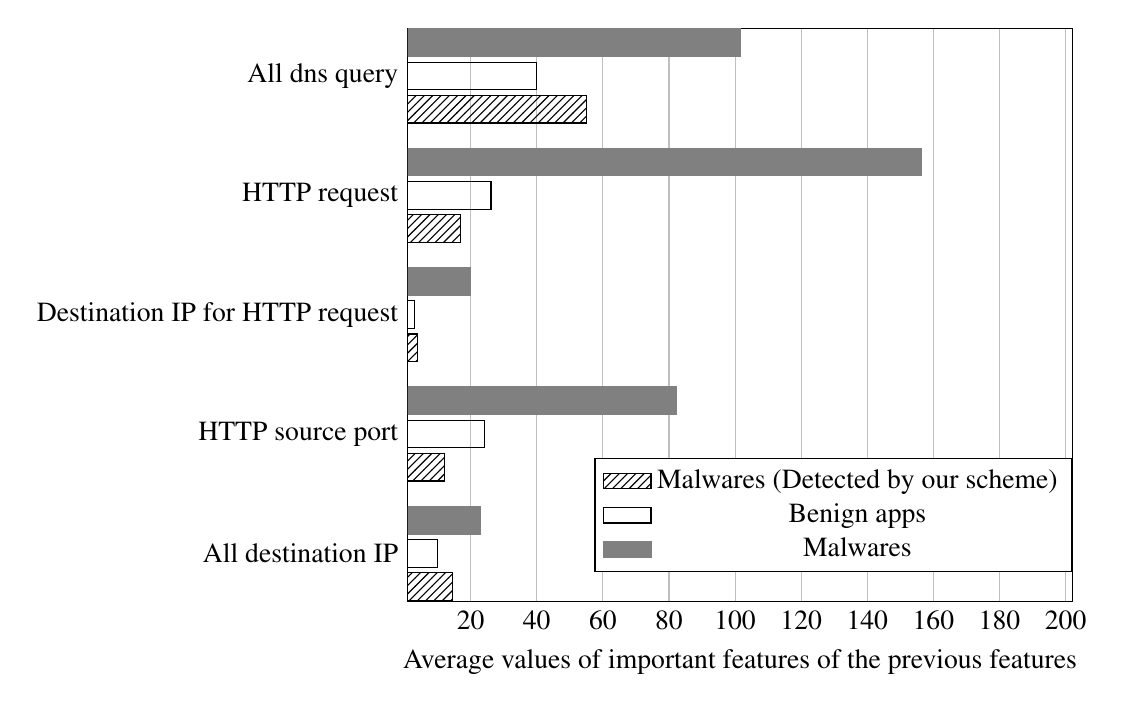
\begin{tikzpicture}
\begin{axis}[
  enlarge y limits=0.1,
  enlarge x limits=0.01,
  % ylabel=Percentage (\%),
  xlabel=Average values of important features of the previous features,
  tickwidth=0pt,
  scale only axis,
  % enlarge x limits=0.2,
  legend style={
    at={(1.0,0.25)},
    % anchor=north,legend columns=-1
  },
  xmax=200,
  xbar,
  area legend, % 長方形の凡例
  % ytick=data,
  % bar width=0.1, % 棒グラフの幅
  symbolic y coords={
    % 0,
    All destination IP,
    HTTP source port,
    Destination IP for HTTP request,
    HTTP request,
    All dns query
  },
  xmajorgrids = true,
  % ytick distance=0.2,       % <-- added
  % ymin=0, ymax=1, % x軸方向の範囲
  % xmajorgrids=false
  ] 
  \addplot [pattern=north east lines] coordinates { % Malwares (Detected by our scheme)
      (14.45,All destination IP)
      (11.99,HTTP source port)
      (3.942,Destination IP for HTTP request) 
      (17.04,HTTP request) 
      (55.08,All dns query) 
      % \label{A}
    };

  \addplot []  coordinates { % (Benign)
      (9.942,All destination IP)
      (24.27,HTTP source port)
      (3,Destination IP for HTTP request) 
      (26.16,HTTP request) 
      (39.94,All dns query) 
      % \label{B}
    };

  \addplot [gray, fill] coordinates { % (Malwares)
      (22.96,All destination IP)
      (82.17,HTTP source port)
      (20.05,Destination IP for HTTP request) 
      (156.48,HTTP request) 
      (101.76,All dns query) 
      % \label{C}
    };
    % \addplot [] coordinates {(0.307,Benign apps) (0.769,Malwares)};
    \legend{Malwares (Detected by our scheme), Benign apps, Malwares}
  \end{axis}
% \begin{customlegend}[legend columns=-1,legend style={draw=none,column sep=1ex},legend entries={Malwares,C,$d$}]
    % \addlegendimage{red,fill=black!50!red,area legend}
    % \addlegendimage{red,fill=black!50!red,sharp plot}
    % \addlegendimage{red,fill=black!50!red,mark=*,sharp plot}
    % % \addlegendimage{red,fill=black!50!red,ybar,ybar legend}
    % \end{customlegend}
\end{tikzpicture}
\end{document}


% \begin{document}
% \begin{tikzpicture}
% \begin{axis}[
% title=Some fancy benchmark data,
% xbar,
% y axis line style={
% draw=none,          % (<-- changed)
% },
% axis x line=none,
% tickwidth=0pt,
% enlarge y limits=0.2,
% enlarge x limits=0.02,
% symbolic y coords={
% Intel Xeon E5630,
% AMD Turion II Neo N54L,
% Intel i7 3632QM%
% },
% nodes near coords,
% nodes near coords style={
% /pgf/number format/precision=4,
% },
% ytick distance=1,       % <-- added
% ]
% \addplot coordinates {
% (0.155,AMD Turion II Neo N54L)
% (0.087,Intel i7 3632QM)
% (0.134,Intel Xeon E5630)
% };
% \addplot coordinates {
% (0.078,AMD Turion II Neo N54L)
% (0.047,Intel i7 3632QM)
% (0.069,Intel Xeon E5630)
% };
% \legend{
% prod1,
% prod2,
% }
% \end{axis}
% \end{tikzpicture}
% \end{document}

